\section{Porting Costs Evaluation}

% What I want to say in this section:
%   - I want to take the model of Tanaka and map my timeline on it (maybe merge
%   the model with [1])
%   - I want to talk about the porting tasks
%     - which was most time consuming
%     - which of them were repetitive and added little value
%     - etc
%   - I want to talk about the human and development factors as described in [1]
%   - talk about environment disparity and program factors; and how did this
%   affect the costs
%   - Finally I need to understand the equations for porting costs evaluation
%   and estimation in order to compare the resluts (and maybe talk about the
%   porting productivity index)
%   - I don't know if I should place it here or in implementation chapter but
%   I would like to have a table with portability impedimets,reason for changes,
%   details of changes and need for change in future porting. They do so in
%   Tanaka et al
%
% LucianM proposed to talk about some aspects of the program to be ported as:
%   - size
%   - content
%
% The Tanaka+Hakuta model mapped on our timeline will be presented in a table.
% The indices from Hakuta([1]) will be presented in different subsection (idk).
%
% [1] "A study of Software Portability Evaluation"

In this section we present the costs associated with the porting process
described in the previous section. First we divide our work in tasks that can
be individually evaluated and later we discuss the factors that affected our
cost evaluation.

\subsection{Man-days costs}

In order to have an accurate cost evaluation of the porting process, we divided
our process into multiple subprocesses that can easily be evaluated using the
tracking created during the porting. We use man-days to evaluate the
cost for each subprocess because the tracking was done each week rather than
each day.

The anatomy of the porting process, as described in Tanaka et al.~\cite{b1}
Hakuta and Ohminami~\cite{b2} and Kanai et al. ~\cite{b4} with modification as
per our project needs has the following structure:
\begin{itemize}
    \item Advance preparations
        \begin{itemize}
            \item Surveying development environment
            \item Surveying target OS
            \item Surveying program for porting
            \item Surveying documentation
            \item Adjusting development environment
            \item Adjusting target environment
            \item Initial source code modifications
        \end{itemize}
    \item Building for target environment
        \begin{itemize}
            \item File-making
            \item Installation on remote environment
            \item Reviewing inconsistencies between source and remote environments
            \item Solving problems with external dependencies
            \item Create testing infrastructure
        \end{itemize}
    \item Testing
        \begin{itemize}
            \item Testing in simulated environment
            \item Testing in target environment
        \end{itemize}
    \item General duties
        \begin{itemize}
            \item Documentation
            \item Progress tracking
            \item Discussions
        \end{itemize}
\end{itemize}

Here we need a paragraph that clarifies some of the porting subprocesses.

This structure assumes that porting is a linear process, which is not the case.
Many tasks are repetitive between different stages of the project. For example
file-making occurs before and after testing in target environment takes place,
making it hard to accurately track each subtask. For this reason table
~\ref{tab:manHoursEvaluation} does not track the exact hours or days spent
on a specific subtask. It rather presents in how many days a specific subtask
was finished, even if that subtask took one or two hours of that day. Finally,
the last column of the table presents the number of days to finish a subtask
relative to the total number of days.

\begin{table*}
\centering
\begin{tabular}{ |l *{5}{|l}| }
\hline
Porting task & Subtasks & Man-hours & Relative man-hours/subtask (\%) & Relative man-hours/task (\%)\\
\hline
\multirow{7}{5em}{Advance preparations} & Surveying development environment & 15 & 4.16 & \multirow{7}{5em}{14.35}\\
& Surveying target OS & 5 & 1.38 &\\
& Surveying program for porting & 3 & 0.83 &\\
& Surveying documentation & 5 & 1.38 &\\
& Adjusting development environment & 10 & 2.77 &\\
& Adjusting target environment & 13.8 & 3.83 &\\
& Initial source code modifications & 0 & 0 &\\
\hline
\multirow{5}{5em}{Building for target environment} & File-making & 67.56  & 18.76  & \multirow{5}{5em}{32.71} \\
& Installation on remote environment & 15.26 & 4.23 &\\
& Reviewing inconsistencies between source and remote environments & 23.03 & 6.39 &\\
& Solving problems with external dependencies & 12 & 3.33 &\\
\hline
\multirow{2}{5em}{Testing} & Testing in simulated environment & 33.35  & 9.26 & \multirow{2}{5em}{24.53} \\
& Testing in target environment & 55 & 15.27 &\\
\hline
\multirow{3}{5em}{General duties} & Documentation & 30  & 8.33  & \multirow{3}{5em}{28.26} \\
& Progress tracking & 12 & 3.33 &\\
& Discussions & 60 & 16.66 &\\
\hline
\multirow{1}{5em}{Total} & & 360  & 100 & \multirow{1}{5em}{100}\\
\hline
\end{tabular}
\caption{Man-days evaluation for porting tasks}
\label{tab:manHoursEvaluation}
\end{table*}

As seen from the table the most time consuming subtask are the following:
discussions, incosistencies reviewing, installation on remote environment and
file-making. The amount of time spent on these tasks is different. While
discussions and inconsistencies reviewing were planned during the day, taking
a predefined amount of time, installation on remote environment and file-making
were repetitive and sporadic tasks. However this does not decrease the
importance of the later tasks, they were time consuming because they helped us
to achieve other tasks, mainly testing tasks.

Another thing that stands out is that we spent zero days on initial source code
modifications. This happened because the code base was too unfamiliar in order
to make source code modifications from the start. The first source code
modifications were present in the reviewing inconsistencies stage because the
toolchain helped us to discover the code zones to be changed.

\subsection{Factors of porting costs}

While porting costs, in our case man-days, are determined dirctly by program size and
content, other factors and impediments as human experience and environment
disparities must be taken into consideration.

To determine the impact some of these factors had on our porting process, we
use the indices described in Hakuta and Ohminami ~\cite{b2} that give
a quantitative influence of porting factors and impediments.

\subsubsection{Portability Impediment Index}

The first index that we compute is the portability impediment index, this will
show us how portable was the porgram we ported and how many difficulties did
we meet in our porting process. The index is computed using the following
formula: $\alpha_p = \eta * \sum_{n=1}^{12} \omega_i S_i$, where $\eta$ is a
portability design index, $\omega_i$ is the weight assigned to each factor and
$S_i$ is 1 when the impediment $i$ exists, otherwise is 0. In our case $eta$
has a value of 2, meaning that "the non-portable parts of the program are not
localized, but the correspondence of program codes to their functions is
clarified". For simplicity we will assume that $\omega_i$ is 0 if the impediment
was insignificant, 0.5 if the impediment had a normal difficulty and 1 if the
impediment was hard to solve. In our porting we discovered the following
portability impediments:
\begin{itemize}
    \item Difference in compiler specification (S8)
    \item Scope of library support (S9)
    \item Implementation-dependent libraries (S10)
    \item Difference in operating system interface (S12)
\end{itemize}

It can be noted that we added an additional impediment inexistent in Hakuta and
Ohminami's list~\cite{b2}, namely S12, which can be placed in the "OS disparity"
category.

Given these impediments the portability impediment index has the following
value: $\alpha_p = 2 * (0.5 * S8 + 1 * S9 + 1 * S10 + 0.5 * S12) = 6$. The
maximum value for $\alpha_p$ is 36 as seen in Figure~\ref{fig:PII}. Our PII is
achieved because there were
no differences between processor architecture (S1~S5), little difference between
source and target OSes (S6, S7, S12) and a major difference in language processor
(S8~S11). The application was written in C++ and the port was between two Linux
versions, which highly decreased the impediments we could have faced. The
degree of portability of the program to be ported is highlighted in Figure
~\ref{fig:PII}, being very close to the optimal value.

\begin{figure}
    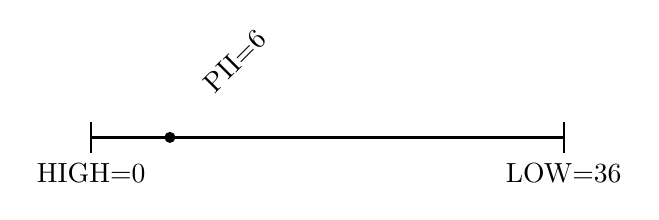
\begin{tikzpicture}[
        dot/.style = {circle, fill=black,inner sep=0pt, minimum size=4pt},
        every label/.append style = {inner sep=0pt, rotate around={45:(-0.5,1.5)}},
            thick      
    ]
        \draw (0,0.2) -- + (0,-0.4) node[below] {HIGH=0};
        \draw (6,0.2) -- + (0,-0.4) node[below] {LOW=36};
        \draw[thick] (0,0) -- node[below=2mm] {} + (6,0);
        \node[dot,label={PII=6}] at (1,0) {};
    \end{tikzpicture}

    \caption{Portability Impediment Index}
    \label{fig:PII}
\end{figure}


\subsubsection{Human Factors Index}

Software programs are byproducts of human
activities than incorporate our problem-solving capabilities, cognitive aspects
and social interaction ~\cite{b3}, therefore it is vital to understand what role
did the human factors play in our porting so that we can assess the quality of
the porting process. 

The index $\alpha_h$ is defined as $\sum_{n=1}^{5} H_i$, where $H_i$ are the
human factors presented in ~\cite{b2}. Their values range from -2 which reflects
the maximum productivity while 2 reflects the minimum productivity. Therefore
in our case $\alpha_h = 2 + (-1) + 2 + 1 + 2 = 6$. As seen in Figure
~\ref{fig:HFI}, the HFI has a score very close to the lowest possible score.
Indeed, the human factor played a major role in our porting process, let us
analyze each factor and see what went wrong.

\begin{figure}
    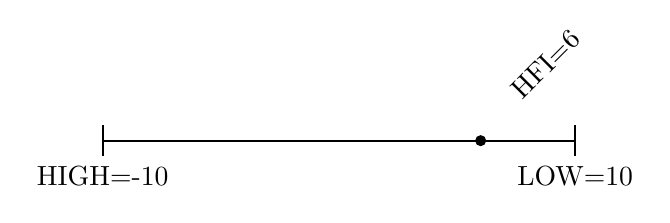
\begin{tikzpicture}[
        dot/.style = {circle, fill=black,inner sep=0pt, minimum size=4pt},
        every label/.append style = {inner sep=0pt, rotate around={45:(-0.5,1.5)}},
            thick      
    ]
        \draw (0,0.2) -- + (0,-0.4) node[below] {HIGH=-10};
        \draw (6,0.2) -- + (0,-0.4) node[below] {LOW=10};
        \draw[thick] (0,0) -- node[below=2mm] {} + (6,0);
        \node[dot,label={HFI=6}] at (4.8,0) {};
    \end{tikzpicture}

    \caption{Human Factors Index}
    \label{fig:HFI}
\end{figure}

\textit{Knowledge about the program to be ported functions and structures (H1)} 
As this was my first interaction with the program to be ported it was hard to
familiarize with its functions and structures, therefore I had no experience
whatsoever with the use cases of the program. This resulted in the inability to
easily solve the porting problems that appeared in our way.

\textit{Knowledge about the hardware and OS of the target system (H2)}
Hardware disparities were not a big concern in our porting as we used a portable
operating system and programming language that abstracted out hardware problems.
Therefore the focus was on the target operating system. Our porting moved the
program from an older version of Linux to a newer one. This helped us as we
did not have to learn the peculiarities of another operating system so that we
could finish our porting. However there were some problems that we faced
regarding the target operating system that we solved relatively straight
forward.

\textit{Knowledge and experience in the area of software porting (H3)}
As the experience of software porting was lacking there were many situations
and problems that could have been solved better, for example: doing better
tracking of the porting process, putting more effort in technical discussions
in order to better understand the problems, etc.

\textit{Knowledge of and experience with the language and program to be ported
in use(H4)}
The experience with the programming language (C++) helped us to grow the
productivity of the porting process as we did not have to care about low-level
impediments as endianness or data alignment. However we did have problems with
the language specification between different compilation toolchains that costed
us a whole week to solve. Finally, the experience with program to be ported in
use was lacking.

\textit{Knowledge about the functions and usage of tools used in the development
and testing environment (H5)}
While working in the development and testing environments we used a considerable
number of technologies, some of them being either new or not trivial to work
with. Here is a short list of these technologies: QEMU networking, SCons build
system, Perforce versioning system and internal tools as packaging system. (are
we allowed to mention these things, i dont see a problem in that tbh)

In retrospect, it seems that if the human factor index had a better score, maybe
the porting process would have lasted less and the problems we faced would not
even occur.

\subsubsection{Environmental Factors Index}

The index $\alpha_e$ is defined as $\sum_{n=1}^{3} E_i$, where $E_i$ are the
following environmental factors as presented in~\cite{b2}:
\begin{itemize}
    \item Development environment (E1)
    \item Unit test environment (E2)
    \item System test environment (E3)
\end{itemize}

In our porting we did not use any kind of unit testing so we will discard E2
from our discussion. As for H1~H5, the values for E1~E3 range between -2 and 2,
-2 being the best score for $E_i$, while 2 being the worst.

In the development environment we had no documentation describing the compiling
and linking procedures and no documentation regarding the environment dependent
components that we need to modify in order to move the code to a new
environment. We modified the code and the build system by trial and error. This
reduces the score for E1 as this strategy might not always work or it could take
an unsatisfactory amount of time for large and complicated systems. However
we managed to understand the peculiarities of the development environment and
get the first builds available for testing in two or three weeks, that is less
than 25\% of our porting time, which is an acceptable value.

In the testing environment we had test programs and tools available such as
simulators and debuggers, furthermore the file transfer and conversion tools
were available from the start of the project. This facilitated the testing of
our program to be ported by allowing us to focus on the porting inconsistencies
rather than on testing infrastructure. Things were not perfect however, we did
have problems with the testing infrastructure that we solved in a short period
of time.

That being said, the environmental factors index has the following value in our
case: $\alpha_e = 0 + NA + -1 = -1$. As seen in Figure~\ref{fig:EFI} we are in the
satisfactory half of the index, meaning that even if we had some difficulties
setting and understanding the development and testing environment, we managed
to work with them in order to achieve our goals.

\begin{figure}
    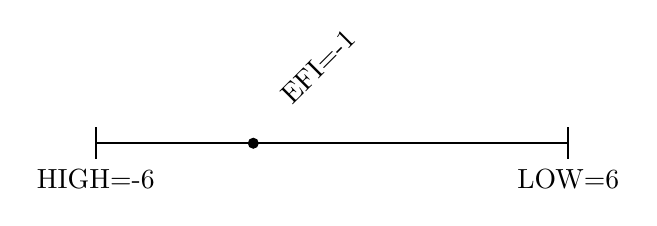
\begin{tikzpicture}[
        dot/.style = {circle, fill=black,inner sep=0pt, minimum size=4pt},
        every label/.append style = {inner sep=0pt, rotate around={45:(-0.5,1.5)}},
            thick      
    ]
        \draw (0,0.2) -- + (0,-0.4) node[below] {HIGH=-6};
        \draw (6,0.2) -- + (0,-0.4) node[below] {LOW=6};
        \draw[thick] (0,0) -- node[below=2mm] {} + (6,0);
        \node[dot,label={EFI=-1}] at (2,0) {};
    \end{tikzpicture}

    \caption{Environmental Factors Index}
    \label{fig:EFI}
\end{figure}

Do we want to measure porting productivity index and porting costs using that
weird equation?
